\section{Dutch Grand Prix}

\subsection{Circuit Analysis}

\textbf{Circuit Name:} Circuit Zandvoort (Zandvoort, Netherlands) \\
\textbf{Length:} 4.259 km - \textbf{Laps:} 72 - \textbf{Total Distance:} 306.587 km

\begin{figure}[H]
    \centering
    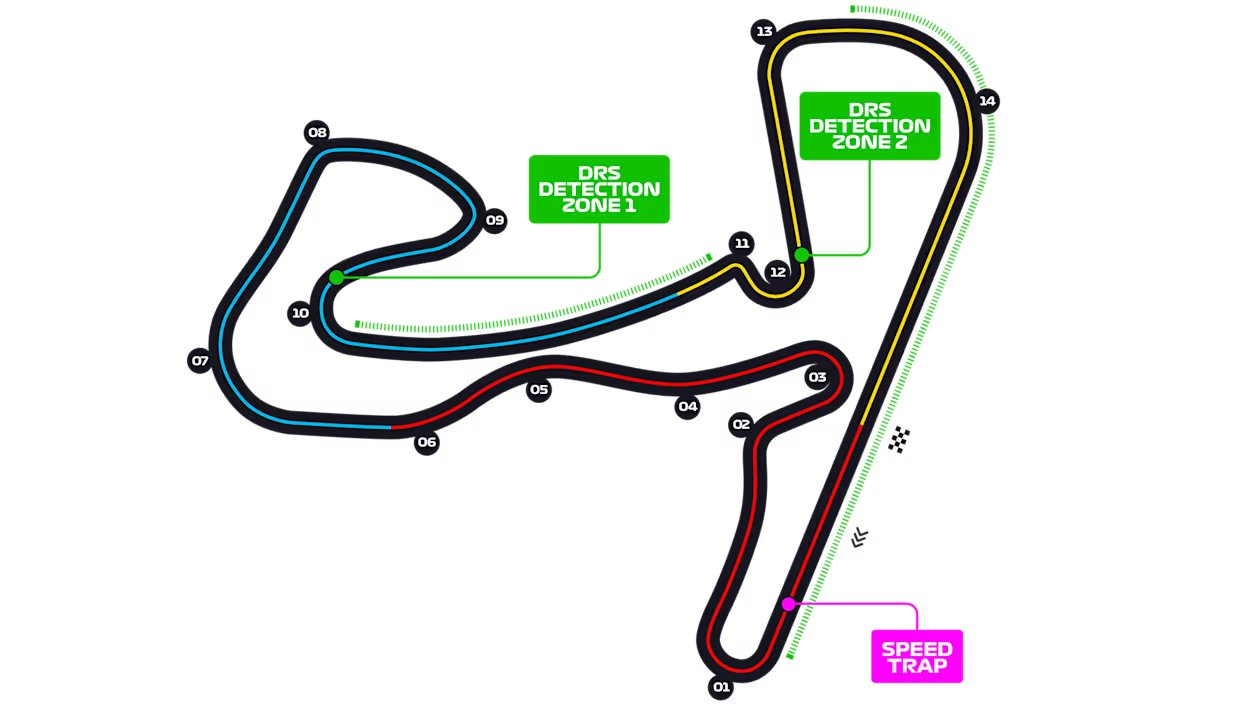
\includegraphics[width=0.75\linewidth]{images/15.Netherlands_Circuit.jpg}
\end{figure}

\begin{itemize}
    \item \textbf{Lap Record} : 1:08.885 (2021, Max Verstappen – Red Bull).
    
    \item \textbf{Number of Corners \& Key Features} : 14 turns (10 right, 4 left). \\
    Famous for banked corners (notably Turn 3 “Hugenholtzbocht” and Turn 14 “Arie Luyendykbocht”). \\
    Narrow track with limited overtaking zones, high emphasis on qualifying.
    
    \item \textbf{Braking Zones \& Traction} : Heavy braking into Turn 1 (Tarzanbocht) is the prime overtaking spot. \\
    Strong traction needed out of the banked final corner to maximize speed on the main straight.
    
    \item \textbf{DRS \& Overtaking} : Two DRS zones (main straight, between Turns 10 and 11). \\
    Overtaking difficult outside of Turn 1 due to narrow layout.
    
    \item \textbf{Tyre Degradation \& Strategy} : High-load corners stress tyres. \\
    Two-stop strategies standard, with high wear on soft compound.
    
    \item \textbf{Weather \& Environment} : Coastal winds and sand from the dunes reduce grip. \\
    Track evolution is significant, demanding constant adaptation.
\end{itemize}

\textbf{Strategic Summary :} Zandvoort rewards qualifying performance, tyre management, and aerodynamic efficiency. The narrow layout limits overtaking, making pit strategy and track position crucial.

\subsection{Race Analysis}

\textbf{Date:} 25 August 2024 — 15:00 local time 

\begin{itemize}
    \item \textbf{Qualifying Summary} : \textbf{Pole Position:} Lando Norris (McLaren) – 1:09.673. \\
    Grid: Verstappen 2nd, Piastri 3rd, Russell 4th. \\
    Hamilton only 14th due to a three grid places penalty, Albon disqualified from qualifying.
    
    \item \textbf{Race Summary} : \textbf{Winner:} Lando Norris (McLaren) — his first hat-trick (pole, win, fastest lap). \\
    \textbf{Podium:} 1. Norris - 2. Verstappen - 3. Leclerc. \\
    No retirements, marking a record fourth GP of the season without DNFs.
    
    \item \textbf{Strategies} : Two-stop race standard across the grid. \\
    - Verstappen led laps 1–17 but lost out on tyre wear. \\
    - Norris retook the lead mid-race and secured victory with fastest lap on the final tour. \\
    - Piastri briefly led (laps 29–32) before dropping behind due to tyre degradation.
    
    \item \textbf{Performance Trends} : 
    \textbf{McLaren:} Norris dominant, Piastri competitive throughout. Clear tyre advantage in long runs. \\
    \textbf{Red Bull:} Verstappen fought hard at home but tyre wear limited his late pace, Pérez underwhelming P6. \\
    \textbf{Ferrari:} Leclerc solid podium, Sainz strong recovery drive to P5. \\
    \textbf{Mercedes:} Russell P7, Hamilton P8 from P14, lacked outright pace compared to rivals. \\
    \textbf{Alpine \& Aston Martin:} Gasly scored again (P9), Alonso took last point (P10).
    
    \item \textbf{Championship Impact} : \textbf{Drivers:} Verstappen 295 pts, Norris 225, Leclerc 192. \\
    \textbf{Constructors:} Red Bull 434, McLaren 404, Ferrari 370, Mercedes 276.
\end{itemize}

\textbf{Key Takeaway :} Lando Norris delivered a flawless weekend, securing pole, victory, and fastest lap for McLaren’s resurgence. Ferrari remained consistent, while Mercedes struggled to extract performance.

\subsection{Link \& Takeaway}

\begin{itemize}
    \item Zandvoort’s narrow layout and banked corners heavily favored track position, McLaren maximized this with Norris’ pole and perfect execution. 
    \item Verstappen’s home GP showed Red Bull’s vulnerability on tyre wear compared to McLaren. 
    \item Ferrari confirmed itself as the “constant podium” team, while Mercedes’ pace deficit became evident. 
    \item The race highlighted McLaren’s transformation into a true championship challenger.
\end{itemize}
